\documentclass[11pt]{article}
\usepackage[utf8]{inputenc} % Para caracteres en espa�ol
\usepackage{amsmath,amsthm,amsfonts,amssymb,amscd}
\usepackage{multirow,booktabs}
\usepackage[table]{xcolor}
\usepackage{fullpage}
\usepackage{lastpage}
\usepackage{enumitem}
\usepackage{floatrow}
\usepackage{multicol}
\usepackage{fancyhdr}
\usepackage{mathrsfs}
\usepackage{wrapfig}
\usepackage[final]{pdfpages}
\usepackage{setspace}
\usepackage{esvect}
\usepackage{calc}
\usepackage{multicol}
\usepackage{cancel}
\usepackage{graphicx}
\graphicspath{ {pictures/} }
\usepackage[retainorgcmds]{IEEEtrantools}
\usepackage[margin=3cm]{geometry}
\usepackage{amsmath}
\newlength{\tabcont}
\setlength{\parindent}{0.0in}
\setlength{\parskip}{0.05in}
\usepackage{empheq}
\usepackage{framed}
%\usepackage{newtxmath}
\usepackage{euscript}
\DeclareMathAlphabet{\mathpzc}{T1}{pzc}{m}{it}
\usepackage[most]{tcolorbox}
\usepackage{xcolor}
\colorlet{shadecolor}{orange!15}
\parindent 0in
\parskip 12pt
\geometry{margin=1in, headsep=0.25in}
\theoremstyle{definition}
\newtheorem{defn}{Definition}
\newtheorem{reg}{Rule}
\newtheorem{exer}{Exercise}
\newtheorem{note}{Note}
\newcommand{\volume}{{\ooalign{\hfil$V$\hfil\cr\kern0.08em--\hfil\cr}}}
\newcommand{\parr}{\mathbin{\|}} % Parralel Symbol
\begin{document}
\setcounter{section}{4}%Section we want -1
\setcounter{page}{41} %Page we want
\setcounter{equation}{43}%Equation we want -1
\def\thepart{\arabic{part}}
\setcounter{part}{8}
\numberwithin{equation}{part}

 \pagestyle{fancy}
\fancyhf{}
\rhead{Section 8:  Electromagnetic Propulsion - Unsteady "Pulsed" Electric Propulsion}
\rfoot{Page \thepage}
\thispagestyle{empty}

\begin{center}
{\LARGE \bf Section 8:  Electromagnetic Propulsion}\\
{\large AE435}\\
Spring 2018
\end{center}
\vspace{5mm}
\section{Unsteady "Pulsed" Electric Propulsion}
\vspace{25mm}
\tableofcontents
\newpage
Unsteady Electromagnetic Acceleration, often called "Pulsed" EP.
 
During WWII the Germans attempted development of an artillery weapon using an approach called the electromagnetic railgun, using jxB force.
 
 
 
  \begin{center}
 \vspace{30mm}
 \textbf{Figure 6: Rail Gun}
 \end{center}
 
 
Magnetic energy, recall Faraday's law:
 
Suppose we clamp the projectile and close the switch, producing a time-varying current in the rails and through the projectile.  From Faraday's law, this produces a voltage in the LC circuit, and a power VJ, which when integrated in time, using (2.94) and (2.96):
 
  \begin{equation*}
\begin{aligned}
\nabla \times \vv{E} &= \frac{\partial \vv{B}}{\partial t} \\ \\
\nabla \times \vv{B} &= \mu_o \, \vv{j}
\end{aligned}
\end{equation*}
 
gives a magnetic energy:
  \begin{equation}
\begin{aligned}
E_{\text{magnetic}} = \int_{\volume} \, \frac{B^2}{2 \, \mu_o} \, \mathrm{d} \volume
\end{aligned}
\end{equation}
over the Bfield volume.
 
The quantity         $\frac{B^2}{2 \, \mu_o}$             	is called the magnetic energy density $[J/m^3]$.  Note these units are the same as $[N/m^2]$ and this quantity is also referred to as the "magnetic pressure".
 
From integral form of Faraday's law: $\varepsilon mf = -\frac{\partial \Phi}{\partial t}$
 
   \begin{equation*}
\begin{aligned}
\Phi = \text{Flux} = \int_S \, \vv{B} \cdot \hat{n} \, \mathrm{d}A
\end{aligned}
\end{equation*}
 
Since $B \sim J$, we can write:

  \begin{equation}
\begin{aligned}
\Phi \equiv L \, J
\end{aligned}
\end{equation}
 
where  L is the self inductance, L is a measure of the magnetic energy that can be stored in a system.  The energy required to create current J in the circuit is then:
 
   \begin{equation}
\begin{aligned}
E_{\text{magnetic}} = \frac{1}{2} \, L \, J^2
\end{aligned}
\end{equation}
 
We now move part of the circuit, e.g., the projectile, by $\mathrm{d}x$, changing the energy by $\mathrm{d}E_{\text{magnetic}}$, which is equivalent to $F_{\text{mag}}$ $\mathrm{d}x$.

Thus, assuming uniform current:
 
   \begin{equation}
\begin{aligned}
F_{\text{mag}} = \frac{\mathrm{d} E_{\text{mag}}}{\mathrm{d} x} = \frac{\mathrm{d} }{\mathrm{d} x} \bigg(\frac{1}{2} \, L \, J^2\bigg) = \frac{1}{2} \, \frac{\mathrm{d} L}{\mathrm{d} x} \, J^2 = \frac{1}{2} \, L' \, J^2
\end{aligned}
\end{equation}
 
For a coaxial railgun (coaxial cylinders), of length x:
 
   \begin{equation}
\begin{aligned}
L = \frac{\mu_o}{2 \, \pi} \bigg[\ln \frac{r_a}{r_c}\bigg]\,x
\end{aligned}
\end{equation}
 
Thus $F_{\text{mag}}$:
 
   \begin{equation}
\begin{aligned}
F_{\text{mag}} = \frac{1}{2} \, \frac{\mu_o}{2 \, \pi} \, \ln \bigg( \frac{r_a}{r_c}\bigg)\, J^2 = \frac{\mu_o \, J^2}{4 \, \pi} \, \ln \bigg( \frac{r_a}{r_c}\bigg)
\end{aligned}
\end{equation}
 
For rectangular rails, width b, thickness c, separation d:
 
   \begin{equation}
\begin{aligned}
L = 0.4 \, \bigg[ \frac{3}{2}x + x \ln \frac{d}{b+c} - d + 0.22(b+c)\bigg]\times 10^{-6} \qquad [\text{Henrys}]
\end{aligned}
\end{equation}

  \begin{equation}
\begin{aligned}
\frac{\mathrm{d} L}{\mathrm{d} x} = L' = 0.6 + 0.4 \, \ln\frac{d}{b+c} \qquad \bigg[\frac{\mu \, H}{m}\bigg]
\end{aligned}
\end{equation}
 
 
For square "thin" rails: $c \rightarrow 0$
 
   \begin{equation*}
\begin{aligned}
L' = 0.6 \qquad \bigg[\frac{\mu \, H}{m}\bigg]
\end{aligned}
\end{equation*}
 
Thus the force is:
 
   \begin{equation}
\begin{aligned}
F = \frac{1}{2} \, L' \, J^2 = 0.3 \times 10^{-6} J^2 = 0.3 \, J^2 \, [kA]
\end{aligned}
\end{equation}
 
 \begin{framed}
\textbf{Example: }Consider a 1 kg projectile traveling along square rails for 10m. The projectile has an exit velocity of 3000 m/s. Find the acceleration, current, power, impedance, voltage and the resulting muzzle energy.

The acceleration is
  \begin{equation*}
\begin{aligned}
a = \frac{v^2}{2 \, l} = \frac{3000^2}{20} = 4.5 \times 10^5 \quad [m/s^2]
\end{aligned}
\end{equation*}
so the force is
  \begin{equation*}
\begin{aligned}
F = ma = 4.5 \times 10^5 \quad [N]
\end{aligned}
\end{equation*}
Recall that the force for square railways is...
  \begin{equation*}
\begin{aligned}
F = \frac{1}{2} \, L' \, J^2 = 0.3 \times 10^{-6} J^2 = 0.3 \, J^2 \, [kA]
\end{aligned}
\end{equation*}
Setting this equal to the force that we calculated, we can computer the current, J.
  \begin{equation*}
\begin{aligned}
4.5 \times 10^5 \quad [N] = 0.3 \, J^2 \, [kA] \rightarrow J = 1220 \, [kA] = 1.22 \, [MA]
\end{aligned}
\end{equation*}
Power:
   \begin{equation}
\begin{aligned}
P = \frac{1}{2} \, F \, u_e = J^2 \, Z = \frac{1}{4} \, L' \, J^2 \, u_e
\end{aligned}
\end{equation}
The electromagnetic imepedance, $Z_{em}$:
  \begin{equation}
\begin{aligned}
Z_{em}=\frac{1}{4} \, L' \, u_e
\end{aligned}
\end{equation}
  \begin{equation*}
\begin{aligned}
Z_{em}= \frac{1}{4} \, 0.6\times10^{-6} \, \cdot 3000 = 0.45 \, [m \Omega]
\end{aligned}
\end{equation*}
thus the voltage, $V_o$:
  \begin{equation*}
\begin{aligned}
V_o = J\,Z = 550 \, [V]
\end{aligned}
\end{equation*}
This could be achieved with the Pulse Forming Network.

The resultant Muzzle Energy is
  \begin{equation*}
\begin{aligned}
\frac{1}{2} \, m \, u_e^2 = 4.5 \, [MJ]
\end{aligned}
\end{equation*}
Clearly large heavy bank of capacitors are required.
 \end{framed}
 
  \begin{center}
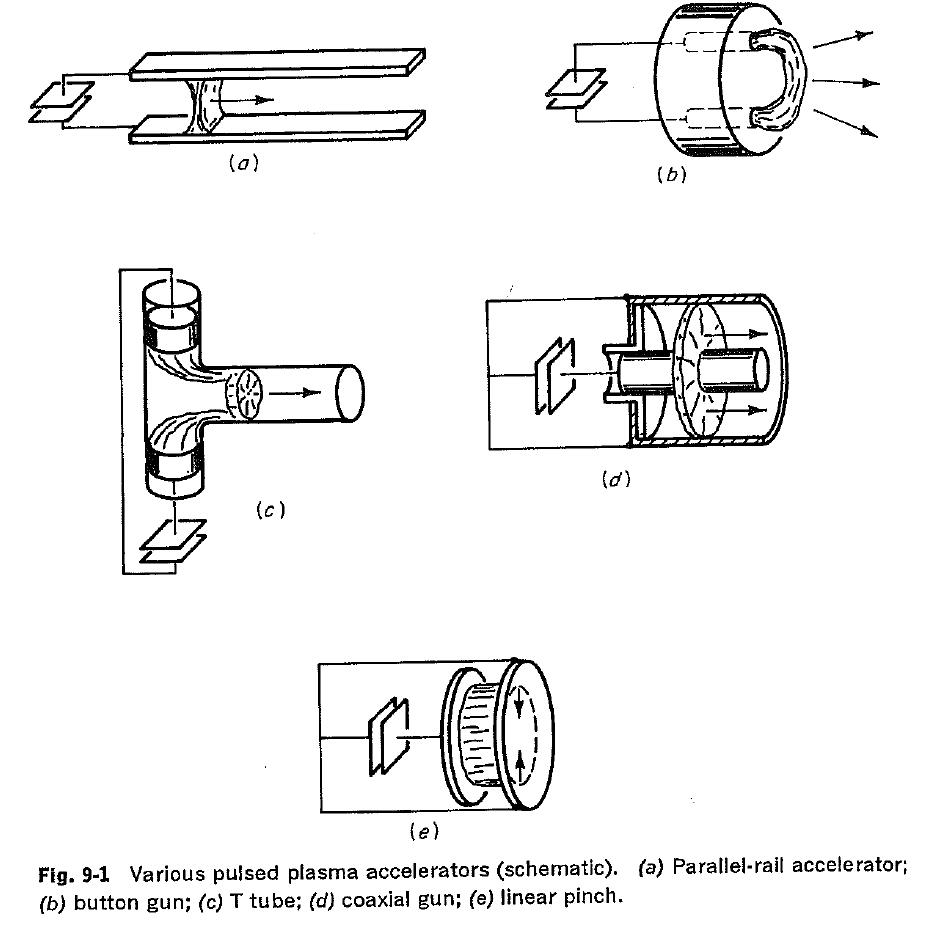
\includegraphics[scale=0.6]{17.png} 
\end{center}

\floatbox[{\capbeside\thisfloatsetup{capbesideposition={right,top},capbesidewidth=6cm}}]{figure*}[\FBwidth]
{\caption{Cross-section diagram of a Pulsed Inductive Thruster. [1] The gas is puffed inward through a central nozzle, towards the flat electromagnetic coil where it is ionized. [2] The plasma (pink) is then accelerated to the rear by the Lorentz force.}}
{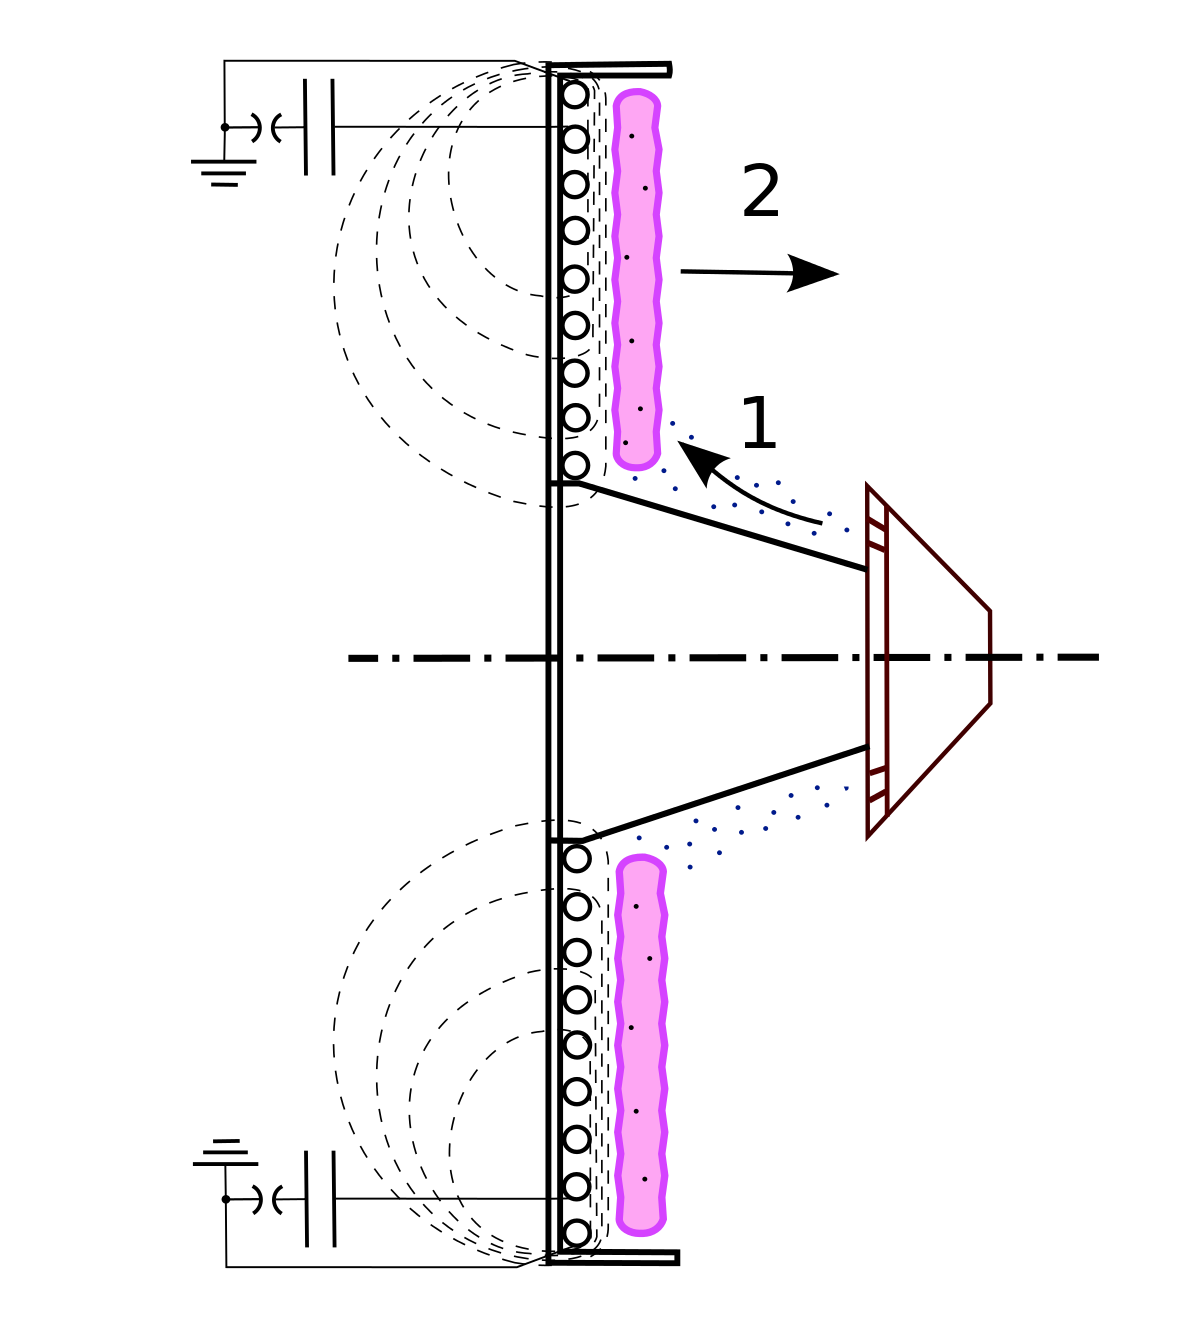
\includegraphics[scale=0.16]{PIT.png}}
 \newpage
\subsection{Slug Model}
The accelerating force as we saw before is:
 \begin{equation*}
\begin{aligned}
F = \frac{1}{2} \, L' \, J^2
\end{aligned}
\end{equation*}

 
Suppose the plasma has mass m, and acts as a compact slug (slug model).  Meaning the mass doesn't change with time (like the railgun).  Then Newton's 2nd law for the equation of motion:
 
 \begin{equation}
\begin{aligned}
\frac{\partial }{\partial t} (m\, \dot{x}) = m \, \ddot{x} = \frac{1}{2}\,L'\,J^2
\end{aligned}
\end{equation}

 
Provided J(t) is known and also        $L'(x) \rightarrow L'(t)$   	, integration gives the velocity and position of the slug vs. time:

\begin{equation*}
\begin{aligned}
\dot{x}(t) \quad \text{and} \quad x(t)
\end{aligned}
\end{equation*}

\newpage
\subsection{Snowplow Model}
If instead, the mass is a gas (not a slug), distributed in front of the plasma current sheet, then the we envision the accelerating plasma current sheet as a "snow plow".   As it propagates and is accelerated downstream, it picks up more mass.   The snowplow model gives:
 
 \begin{equation}
\begin{aligned}
\frac{\partial }{\partial t} (m \, \dot{x}) = m \, \ddot{x} + \dot{m}\, \dot{x}= \frac{1}{2}\,L'\,J^2
\end{aligned}
\end{equation}

 
Again it is straightforward to find velocity,     $\dot{x}$    , and position,    $x$	by numerical integration, $m = \int \dot{m} \mathrm{d}t$.  And for simple cases even analytically.
 
For a pulsed thruster with fill mass density, $\rho = const.$ and area, $A = const.$
Then the snowplowed mass is:

\begin{equation}
\begin{aligned}
m = \rho \, A \, x
\end{aligned}
\end{equation}

 
Thus the force equation is:
 
 \begin{equation}
\begin{aligned}
\frac{\partial }{\partial t} (\rho \, A \, x \, \dot{x}) = \frac{1}{2}\,L'\,J^2
\end{aligned}
\end{equation}

 
If we assume J = const. and L' = const (constant force), we can integrate once to get:
 
 \begin{equation}
\begin{aligned}
m \dot{x} = \frac{1}{2}\,L'\,J^2 \, t
\end{aligned}
\end{equation}

 
The solution of which is :
 
 \begin{equation}
\begin{aligned}
\dot{x} = \sqrt{\frac{\frac{1}{2} \, L' \, J^2}{\rho \, A}}
\end{aligned}
\end{equation}

 
Here,     $\dot{x}$    	, is adjusted by changing $\rho$

\newpage
\subsection{Gasdynamic Model}
 A refinement to the snowplow model is to treat the current sheet as an impermeable surface.  In this case it's like a piston being driven into a gas at high speeds.  A shock wave form upstream of the piston (current sheet) that compresses and accelerates the stationary/stagnant gas.
 
 \begin{center}
\vspace{50mm}
\textbf{Figure 7: Piston moving along u creating a moving schockwave.}
 \end{center}
 
This type of setup can be modeled using unsteady gas-dynamics models, see for example Liepmann and Roshko "Elements of Gas-dynamics".
 
Here we look at efficiency.

In our case, the piston is the current sheet that acts as an impermeable piston that runs into stagnate airflow, compressing the gas. We can consider the current sheet as a very strong shock with a large density jump.

In the Shock Reference frame:
 
 \begin{center}
\vspace{50mm}
\textbf{Figure 8: Current sheet compressing low density gas}
 \end{center}
 
The downstream velocity, u2 is very subsonic, so the flow behind the sheet is essentially stagnant.
 
Total enthalpy is conserved (conservation of energy) across the sheet:
 
 \begin{equation}
\begin{aligned}
h_1 + \frac{u_1^2}{2} = h_2 + \frac{u_2^2}{2}
\end{aligned}
\end{equation}
 \begin{equation*}
\begin{aligned}
a
\end{aligned}
\end{equation*}
%we are taking all the kinetic energy of the gas and converting it into enthalpy at the downstream end.
 \begin{equation}
\begin{aligned}
\frac{u_1^2}{2} = h_2
\end{aligned}
\end{equation}
Now, in the lab frame,  sheet and  snowplowed mass are at $u_1$, so:
 
  \begin{equation}
\begin{aligned}
a
\end{aligned}
\end{equation}
 
The upper limit is 50$\%$ assuming that J  goes  to zero and the electric energy goes to zero ($\frac{1}{2}CV_o^2$)as the accelerated mass exits.
 %This is purely gas dynamic becuase J went to 0 for this model. There is not just energy in the fluid, there is also energy is
 %Why does J=0 for this model? There will still be magnetic and electric energy in the plasma 
 
A major drawback is the need for  a fast valve to puff in the gas.  The valve must operate large number of cycles.  All these devices are characterized by a moving current and B-field pattern.
\end{document}